
%(BEGIN_QUESTION)
% Copyright 2013, Tony R. Kuphaldt, released under the Creative Commons Attribution License (v 1.0)
% This means you may do almost anything with this work of mine, so long as you give me proper credit

Examine this process trend showing the PV, SP, and Output of a loop controller:

$$\includegraphics[width=15.5cm]{i02633x01.eps}$$

Based on what you see here, determine the following:

\begin{itemize}
\item{} Whether this is an open-loop or a closed-loop response
\item{} Whether the controller is (or needs to be) {\it direct-acting} or {\it reverse-acting}
\item{} If possible, identify any problems with the field instrumentation
\item{} If possible, identify any problems with the controller PID tuning
\item{} Qualitatively identify the kind of PID tuning we will need for robust control
\end{itemize}

\underbar{file i02633}
%(END_QUESTION)





%(BEGIN_ANSWER)

This is a {\it closed-loop test}, based on the fact the output signal responds dynamically to the changing process variable, as well as to the step-change in setpoint.

\vskip 10pt

This is a {\it reverse-acting} controller: the output steps up when the setpoint steps up (implying the output would step down if the process variable stepped up).

\vskip 10pt

There do not appear to be any field instrumentation problems revealed in this trend.  A manual-mode (open-loop) test would be more informative in that regard, but it appears as though the process is very quick to respond with no discernable dead time or other lags.

\vskip 10pt
  
The controller tuning is too heavy on proportional action.  We can tell this from the phase shift between PV and output during the oscillations, which is nearly 180$^{o}$.  Excessive integral action would shift the phase of the output wave further to the right (i.e. so that each peak of the output waveform coincided with the zero-crossing of the PV waveform, or very nearly).  The fact that the inverse peaks of the PV and output waves are very nearly aligned tells us that excessive gain (proportional action) is the culprit here.  Another clue is the magnification of noise we see in the output trend compared to the PV trend -- only proportional action or derivative action can cause this, and since we see no sign of excessive derivative action (e.g. output wave leading the PV wave), we can safely say the problem is too much gain.

\vskip 10pt

The process response time (dead time, lag time) seems to be very short, which is a good thing for process control.  We can tell, however, that this is an {\it integrating} process by the way it was able to achieve a new SP value with the old output value.  This means it will exhibit some overshoot with SP changes if there is any integral action.  We may have to do most of the control through proportional action (albeit much less gain than we are using now!), with just enough integral action to handle load changes.

%(END_ANSWER)





%(BEGIN_NOTES)


%INDEX% Process troubleshooting: diagnosing problem via trend recording

%(END_NOTES)


